\documentclass[a4paper,14pt]{extarticle}

\usepackage[utf8x]{inputenc}
\usepackage[T1]{fontenc}
\usepackage[russian]{babel}
\usepackage{hyperref}
\usepackage{indentfirst}
\usepackage{here}
\usepackage{array}
\usepackage{graphicx}
\usepackage{caption}
\usepackage{subcaption}
\usepackage{chngcntr}
\usepackage{amsmath}
\usepackage{amssymb}
\usepackage[left=2cm,right=2cm,top=2cm,bottom=2cm,bindingoffset=0cm]{geometry}
\usepackage{multicol}
\usepackage{multirow}
\usepackage{titlesec}
\usepackage{listings}
\usepackage{color}
\usepackage{enumitem}
\usepackage{cmap}
\usepackage{underscore}

\definecolor{green}{rgb}{0,0.6,0}
\definecolor{gray}{rgb}{0.5,0.5,0.5}
\definecolor{purple}{rgb}{0.58,0,0.82}

\lstdefinelanguage{none}{}

\lstset{
	language={Java},
	inputpath={../generator/src/main/java/com/vaddya/hotelbooking},
	backgroundcolor=\color{white},
	commentstyle=\color{green},
	keywordstyle=\color{blue},
	numberstyle=\scriptsize\color{gray},
	stringstyle=\color{purple},
	basicstyle=\ttfamily\small,
	breakatwhitespace=false,
	breaklines=true,
	captionpos=b,
	keepspaces=true,
	numbers=left,
	numbersep=5pt,
	showspaces=false,
	showstringspaces=false,
	showtabs=false,
	tabsize=4,
	texcl=true,
	extendedchars=false,
	frame=single,
	morekeywords={IF, BIGSERIAL, SERIAL, TEXT, BIGINT, MONEY, BOOLEAN, REFERENCES}
}

\renewcommand{\le}{\ensuremath{\leqslant}}
\renewcommand{\leq}{\ensuremath{\leqslant}}
\renewcommand{\ge}{\ensuremath{\geqslant}}
\renewcommand{\geq}{\ensuremath{\geqslant}}
\renewcommand{\epsilon}{\ensuremath{\varepsilon}}
\renewcommand{\phi}{\ensuremath{\varphi}}
\renewcommand{\thefigure}{\arabic{figure}}
\newcommand{\code}[1]{\texttt{#1}}
\newcommand{\caret}{\^{}}

\titleformat*{\section}{\large\bfseries} 
\titleformat*{\subsection}{\normalsize\bfseries} 
\titleformat*{\subsubsection}{\normalsize\bfseries} 
\titleformat*{\paragraph}{\normalsize\bfseries} 
\titleformat*{\subparagraph}{\normalsize\bfseries} 

\counterwithin{figure}{section}
\counterwithin{equation}{section}
\counterwithin{table}{section}
\newcommand{\sign}[1][5cm]{\makebox[#1]{\hrulefill}}
\newcommand{\equipollence}{\quad\Leftrightarrow\quad}
\newcommand{\no}[1]{\overline{#1}}
\graphicspath{{../pics/}}
\captionsetup{justification=centering,margin=1cm}
\def\arraystretch{1.3}
\setlength\parindent{5ex}
\titlelabel{\thetitle.\quad}

\setitemize{topsep=0.5em, itemsep=0em}
\setenumerate{topsep=0.5em, itemsep=0em}

\begin{document}

\begin{titlepage}
\begin{center}
	Санкт-Петербургский Политехнический Университет Петра Великого\\[0.3cm]
	Институт компьютерных наук и технологий \\[0.3cm]
	Кафедра компьютерных систем и программных технологий\\[4cm]
	
	\textbf{ОТЧЕТ}\\ 
	\textbf{по лабораторной работе}\\[0.5cm]
	\textbf{<<Разработка структуры базы данных>>}\\[0.1cm]
	Базы данных\\[3.0cm]
\end{center}

\begin{flushright}
	\begin{minipage}{0.45\textwidth}
		\textbf{Работу выполнил студент}\\[3mm]
		группа 43501/3 \hfill Дьячков В.В.\\[5mm]
		\textbf{Работу принял преподаватель}\\[5mm]
		\sign[3cm] \hfill Мяснов А.В. \\[5mm]
	\end{minipage}
\end{flushright}

\vfill

\begin{center}
	Санкт-Петербург\\[0.3cm]
	\the\year
\end{center}
\end{titlepage}

\addtocounter{page}{1}

\tableofcontents
\newpage

\section{Цель работы}

Познакомиться с основами проектирования схемы БД, языком описания сущностей и ограничений БД SQL-DDL.

\section{Программа работы}

\begin{enumerate}
	\item Самостоятельное изучение SQL-DDL.
	\item Создание скрипта БД в соответствии с согласованной схемой. Должны присутствовать первичные и внешние ключи, ограничения на диапазоны значений. Демонстрация скрипта преподавателю. 
	\item Создание скрипта, заполняющего все таблицы БД данными.
	\item Выполнение SQL-запросов, изменяющих схему созданной БД по заданию преподавателя. Демонстрация их работы преподавателю.
\end{enumerate}

\section{Теоретическая информация}

\textbf{Язык SQL} (Structured Query Language) -- язык структурированных запросов. Он позволяет формировать весьма сложные запросы к базам данных. В SQL определены два подмножества языка:

\begin{itemize}
	\item \textbf{SQL-DDL} (Data Definition Language) -- язык определения структур и ограничений целостности баз данных. Сюда относятся команды создания и удаления баз данных; создания, изменения и удаления таблиц; управления пользователями и т.д.
	\item \textbf{SQL-DML} (Data Manipulation Language) -- язык манипулирования данными: добавление, изменение, удаление и извлечение данных, управления транзакциями. Функции SQL-DML определяются первым словом в предложении (часто называемом запросом), которое является глаголом: \code{SELECT} (<<выбрать>>), \code{INSERT} (<<вставить>>), \code{UPDATE} (<<обновить>>), и \code{DELETE} (<<удалить>>). 
\end{itemize}

\section{Выполнение работы}

\subsection{Структура базы данных}

\begin{figure}[H]
	\centering
	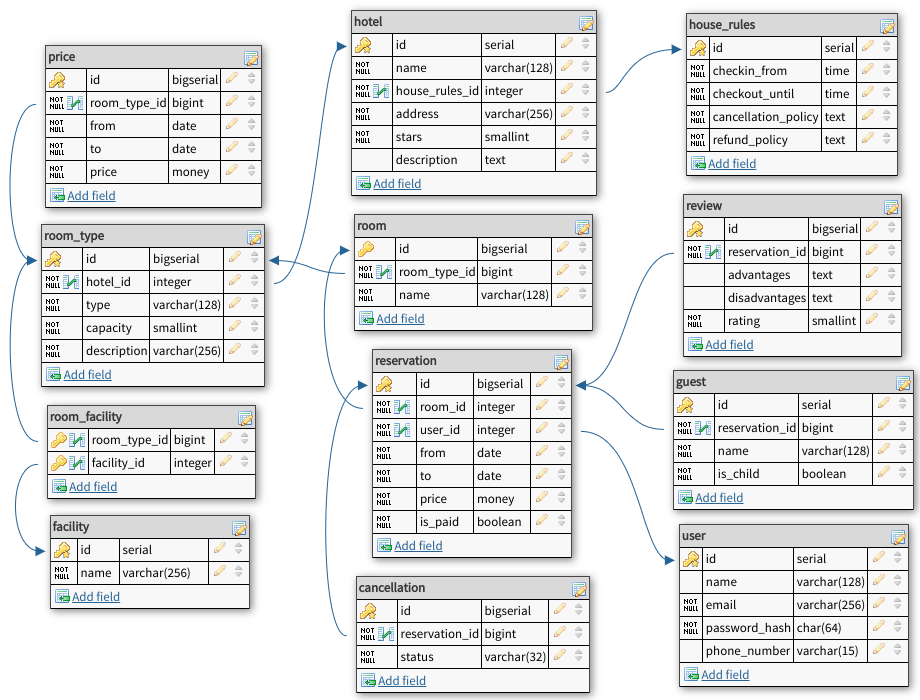
\includegraphics[width=\linewidth]{V1__create}
	\caption{Структура базы данных}
\end{figure}

\subsection{Скрипт создания структуры базы данных}

\lstinputlisting{../../migrations/V1__create.sql}

\subsection{Скрипт заполнения таблиц тестовыми данными}

\lstinputlisting{insert.sql}

\subsection{Изменение структуры базы данных}

По заданию преподавателя схема БД была изменена для удовлетворения следующим требованиям:

\begin{itemize}
	\item Добавить связь со странами и городами
	\item Добавить учет бонусов и штрафов с учетом условий бронирования
\end{itemize}

Были добавлены следующие таблицы:

\begin{itemize}
	\item \code{country} -- хранит 3-символьный код \code{id} и название \code{name} страны.
	
	\item \code{city} -- хранит название \code{name} и 3-символьный код страны \code{country_id}.
	
	\item \code{bonus_penalty} -- хранит условие предоставление бонуса или причину штрафа \code{condition} и соответствующий денежный бонус/штраф \code{price}.
	
	\item \code{bonus_penalty_reservation} -- соотносит бронирование \code{reservation_id} с бонусами/штрафами \code{bonus_penalty_id}.
\end{itemize}

\begin{figure}[H]
	\centering
	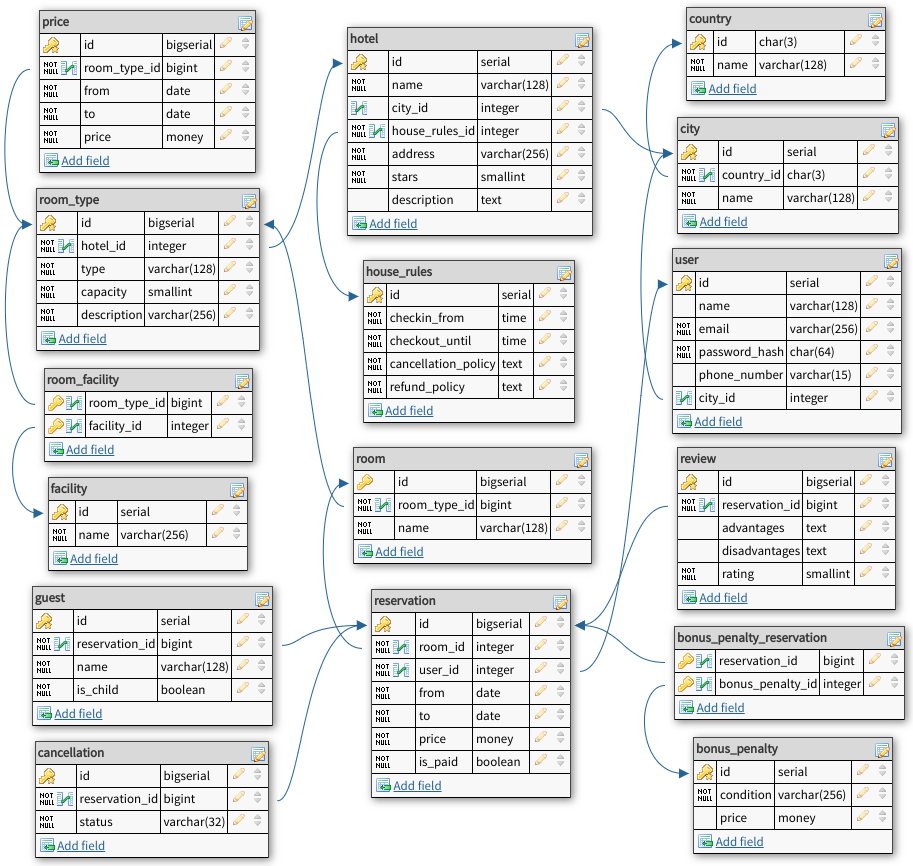
\includegraphics[width=\linewidth]{V2__alter}
	\caption{Структура базы данных}
\end{figure}

Скрипт создания дополнительных таблиц, внесения в них тестовых данных, и изменения существующих:

\lstinputlisting{../../migrations/V2__alter.sql}

\section{Выводы}

В ходе выполнения данной работы были изучены основы создания скриптов на языке SQL. С помощью SQL-DDL описаны структуры разрабатываемой схемы базы данных. С использованием SQL-DML созданные структуры заполнены тестовыми данными. Изучен синтаксис обновления структуры существующей таблицы.

\end{document}
